\documentclass[a4paper,11pt]{article}

%% ── Encodage & Langue ────────────────────────────────────────
\usepackage[T1]{fontenc}
\usepackage[utf8]{inputenc}
%% ── Polices ─────────────────────────────────────────────────
\usepackage[protrusion=false,expansion=false]{microtype}

%% ── Mise en page ─────────────────────────────────────────────
\usepackage[
  a4paper,
  top=2.5cm, bottom=2.5cm,
  left=2.2cm, right=2.2cm,
  headheight=14pt
]{geometry}

%% ── Couleurs ─────────────────────────────────────────────────
\usepackage[dvipsnames,table]{xcolor}
\definecolor{BlueDark}{HTML}{1F3864}
\definecolor{BlueMid}{HTML}{2E75B6}
\definecolor{BlueLight}{HTML}{D6E4F0}
\definecolor{BlueHeader}{HTML}{BDD7EE}
\definecolor{GreenBox}{HTML}{E2EFDA}
\definecolor{GreenBorder}{HTML}{70AD47}
\definecolor{OrangeBox}{HTML}{FCE4D6}
\definecolor{OrangeBorder}{HTML}{ED7D31}
\definecolor{GrayBg}{HTML}{F5F5F5}
\definecolor{CodeBg}{HTML}{F8F8F8}
\definecolor{CodeRed}{HTML}{C7254E}
\definecolor{DarkGray}{HTML}{333333}

%% ── En-tête / Pied de page ───────────────────────────────────
\usepackage{fancyhdr}
\pagestyle{fancy}
\fancyhf{}
\fancyhead[L]{\small\color{BlueMid}\textbf{TD3 : Debugging and Profiling}}
\fancyhead[R]{\small\color{gray}Master CHPS --- Semestre 2, 2025-2026}
\fancyfoot[C]{\small\color{gray}\thepage}
\fancyfoot[L]{\small\color{gray}Yaya Toure}
\fancyfoot[R]{\small\color{gray}Universit\'e}
\renewcommand{\headrulewidth}{0.4pt}
\renewcommand{\headrule}{\hbox to\headwidth{\color{BlueMid}\leaders\hrule height \headrulewidth\hfill}}
\renewcommand{\footrulewidth}{0.4pt}
\renewcommand{\footrule}{\hbox to\headwidth{\color{BlueMid}\leaders\hrule height \footrulewidth\hfill}}

%% ── Titres de sections ───────────────────────────────────────
\usepackage{titlesec}
\titleformat{\section}
  {\color{BlueDark}\Large\bfseries}
  {\color{BlueMid}\rule[-4pt]{3pt}{14pt}\hspace{8pt}\thesection.}
  {6pt}{}
  [\vspace{-4pt}\color{BlueMid}\rule{\linewidth}{0.6pt}\vspace{2pt}]

\titleformat{\subsection}
  {\color{BlueMid}\large\bfseries}
  {\thesubsection.}{6pt}{}

\titleformat{\subsubsection}
  {\color{DarkGray}\normalsize\bfseries}
  {\thesubsubsection.}{4pt}{}

\titlespacing*{\section}{0pt}{18pt}{8pt}
\titlespacing*{\subsection}{0pt}{12pt}{4pt}
\titlespacing*{\subsubsection}{0pt}{8pt}{2pt}

%% ── Tableaux ─────────────────────────────────────────────────
\usepackage{booktabs}
\usepackage{tabularx}
\usepackage{multirow}
\usepackage{array}
\usepackage{colortbl}
\newcolumntype{L}[1]{>{\raggedright\arraybackslash}p{#1}}
\newcolumntype{C}[1]{>{\centering\arraybackslash}p{#1}}
\newcolumntype{R}[1]{>{\raggedleft\arraybackslash}p{#1}}

%% ── Listings (code) ──────────────────────────────────────────
\usepackage{listings}
\lstset{
  basicstyle=\ttfamily\small,
  backgroundcolor=\color{CodeBg},
  frame=single,
  framerule=0pt,
  rulecolor=\color{BlueMid},
  xleftmargin=4pt, xrightmargin=4pt,
  breaklines=true,
  breakatwhitespace=true,
  keepspaces=true,
  showstringspaces=false,
  tabsize=4,
  numbers=left,
  numberstyle=\tiny\color{gray},
  numbersep=6pt,
  commentstyle=\color{gray}\itshape,
  keywordstyle=\color{BlueMid}\bfseries,
  stringstyle=\color{CodeRed},
  identifierstyle=\color{DarkGray},
}
\lstdefinestyle{bash}{
  language=bash,
  basicstyle=\ttfamily\small\color{DarkGray},
  backgroundcolor=\color{GrayBg},
  keywordstyle=\color{BlueMid}\bfseries,
  numbers=none,
}
\lstdefinestyle{cpp}{
  language=C++,
  basicstyle=\ttfamily\small,
  backgroundcolor=\color{CodeBg},
  keywordstyle=\color{BlueMid}\bfseries,
  stringstyle=\color{CodeRed},
  commentstyle=\color{gray}\itshape,
  numbers=left,
  numberstyle=\tiny\color{gray},
}
\lstdefinestyle{output}{
  basicstyle=\ttfamily\footnotesize\color{DarkGray},
  backgroundcolor=\color{GrayBg},
  frame=single,
  framerule=0pt,
  numbers=none,
  breaklines=true,
}

%% ── Boîtes colorées ──────────────────────────────────────────
\usepackage[most]{tcolorbox}
\tcbset{
  base/.style={
    arc=3pt, boxrule=0.8pt,
    left=8pt, right=8pt, top=6pt, bottom=6pt,
    fonttitle=\bfseries\small,
    coltitle=white,
  }
}
\newtcolorbox{successbox}[1][]{
  base, colback=GreenBox, colframe=GreenBorder, #1
}
\newtcolorbox{warningbox}[1][]{
  base, colback=OrangeBox, colframe=OrangeBorder, #1
}
\newtcolorbox{infobox}[1][]{
  base, colback=BlueLight, colframe=BlueMid, #1
}

%% ── Graphiques & TikZ ────────────────────────────────────────
\usepackage{tikz}
\usepackage{pgfplots}
\pgfplotsset{compat=1.18}
\usetikzlibrary{shapes.geometric, arrows.meta, positioning, shadows, backgrounds, patterns}

%% ── Divers ───────────────────────────────────────────────────
\usepackage{graphicx}
\usepackage{enumitem}
\usepackage{amsmath}
\usepackage{amssymb}
\usepackage{float}
\usepackage{caption}
\usepackage{setspace}
\usepackage{parskip}

%% ── Hyperref ─────────────────────────────────────────────────
\usepackage[
  colorlinks=true,
  linkcolor=BlueMid,
  urlcolor=BlueMid,
  citecolor=BlueMid,
  pdfauthor={Yaya Toure},
  pdftitle={TD3 Debugging and Profiling --- Master CHPS},
]{hyperref}

%% ── Commandes utilitaires ────────────────────────────────────
\newcommand{\code}[1]{\texttt{\color{CodeRed}#1}}
\newcommand{\cmd}[1]{\texttt{\color{BlueMid}#1}}
\newcommand{\file}[1]{\texttt{\textit{#1}}}
\newcommand{\result}[1]{\textbf{\color{GreenBorder}#1}}

\setlength{\parindent}{0pt}
\setlength{\parskip}{6pt}

%% ============================================================
\begin{document}
%% ============================================================

%% ── PAGE DE TITRE ────────────────────────────────────────────
\thispagestyle{empty}

\begin{tikzpicture}[remember picture, overlay]
  \fill[BlueDark] (current page.north west)
    rectangle ([yshift=-5cm]current page.north east);
  \fill[BlueMid] (current page.south west)
    rectangle ([yshift=1.5cm]current page.south east);
  \fill[BlueLight, opacity=0.3]
    ([xshift=12cm, yshift=-1cm]current page.north west)
    circle (6cm);
\end{tikzpicture}

\vspace*{0.8cm}

{\color{white}
  \begin{center}
    {\fontsize{13}{16}\selectfont\textsc{Universit\'e --- Master 1 CHPS}}\\[0.15cm]
    {\fontsize{11}{14}\selectfont Semestre 2 --- 2025-2026}\\[0.8cm]
    \rule{0.4\linewidth}{0.5pt}\\[0.6cm]
    {\fontsize{28}{34}\selectfont\bfseries Debugging \& Profiling}\\[0.3cm]
    {\fontsize{18}{22}\selectfont\bfseries TD n\textsuperscript{o}3}\\[0.3cm]
    \rule{0.4\linewidth}{0.5pt}\\[0.6cm]
    {\fontsize{14}{18}\selectfont Optimisation de boucles --- \texttt{ssgemm}}
  \end{center}
}

\vspace{3.5cm}

\begin{center}
\begin{tcolorbox}[
  width=0.72\linewidth,
  colback=white, colframe=BlueMid,
  arc=4pt, boxrule=1.2pt,
  left=16pt, right=16pt, top=12pt, bottom=12pt,
]
  \begin{center}
    {\large\bfseries\color{BlueDark} Yaya Toure}\\[4pt]
    {\small\color{gray} Master 1 CHPS --- Parcours Calcul Haute Performance}\\[4pt]
    {\small\color{gray} Ann\'ee universitaire 2025-2026}
  \end{center}
\end{tcolorbox}
\end{center}

\vspace{1cm}

\begin{center}
\begin{tcolorbox}[
  width=0.88\linewidth,
  colback=BlueLight, colframe=BlueMid,
  arc=3pt, boxrule=0.6pt,
  left=12pt, right=12pt, top=8pt, bottom=8pt,
]
  \small\color{DarkGray}
  \textbf{R\'esum\'e :} Ce rapport pr\'esente les travaux r\'ealis\'es lors du TD3 portant
  sur l'optimisation de transformations de boucles appliqu\'ees \`a la fonction
  \code{ssgemm} (produit matriciel). En s'appuyant sur l'article de r\'ef\'erence
  \textit{Compiler Transformations for High-Performance Computing} (Bacon, Graham \&
  Sharp, 1994), nous avons analys\'e les d\'ependances du nid de boucle, identifi\'e la
  meilleure permutation (\textbf{r\,$\to$\,d\,$\to$\,c}, gain $\times$10--21) et valid\'e
  la l\'egalit\'e du blocage de boucles (\textit{loop tiling}) avec une taille de bloc
  optimale de \textbf{32}, permettant d'atteindre les meilleures performances sur notre
  machine (Cache L1d = 64\,KiB).
\end{tcolorbox}
\end{center}

\vfill

{\color{white}\small\centering
  Universit\'e --- Master CHPS \quad|\quad TD3 Debugging \& Profiling \quad|\quad 2025-2026
}

\newpage
\tableofcontents
\newpage

%% ============================================================
\section{Contexte th\'eorique --- Article de r\'ef\'erence}
%% ============================================================

Ce TD s'appuie sur l'article fondateur de Bacon, Graham \& Sharp (1994),
\textit{``Compiler Transformations for High-Performance Computing''}, publi\'e dans
\textit{ACM Computing Surveys}. Cet article de synth\`ese recense toutes les
transformations que les compilateurs optimisants peuvent appliquer pour maximiser
les performances sur les architectures superscalaires, vectorielles et parall\`eles.

\subsection{Types de d\'ependances (Section 5)}

L'article distingue trois types fondamentaux de d\'ependances entre instructions
$S_1$ et $S_2$ :

\begin{center}
\rowcolors{2}{GrayBg}{white}
\begin{tabular}{L{3.2cm}L{5cm}L{5cm}}
  \toprule
  \rowcolor{BlueHeader}
  \textbf{Type} & \textbf{D\'efinition} & \textbf{Contrainte} \\
  \midrule
  \textbf{Flow dependence} (vraie) & $S_1$ \'ecrit, $S_2$ lit & $S_1$ doit pr\'ec\'eder $S_2$ \\
  \textbf{Anti-d\'ependance}       & $S_1$ lit, $S_2$ \'ecrit & $S_2$ doit suivre $S_1$ \\
  \textbf{Output dependence}       & $S_1$ et $S_2$ \'ecrivent au m\^eme endroit & Ordre d'\'ecriture pr\'eserv\'e \\
  \bottomrule
\end{tabular}
\end{center}

Pour les boucles, ces d\'ependances sont caract\'eris\'ees par des \textbf{vecteurs de
direction} (ex. \texttt{<}, \texttt{=}, \texttt{>}) indiquant la relation entre
it\'erations.

\subsection{M\'etriques de performance (Section 3.1)}

\begin{center}
\rowcolors{2}{GrayBg}{white}
\begin{tabular}{L{2.5cm}L{4cm}L{6.5cm}}
  \toprule
  \rowcolor{BlueHeader}
  \textbf{M\'etrique} & \textbf{D\'efinition} & \textbf{Impact} \\
  \midrule
  \textbf{Q}      & R\'eutilisation registre / chargements m\'emoire & Plus Q est \'elev\'e, moins on charge depuis la m\'emoire \\
  \textbf{Qc}     & R\'eutilisation cache / chargements depuis RAM   & Plus Qc est \'elev\'e, meilleure utilisation du cache \\
  \textbf{Stride} & Distance entre \'el\'ements acc\'ed\'es cons\'ecutivement & Stride-1 = acc\`es contigu = optimal \\
  \bottomrule
\end{tabular}
\end{center}

\subsection{Transformations de r\'eordonnancement (Section 6.2)}

\begin{center}
\rowcolors{2}{GrayBg}{white}
\begin{tabular}{L{4cm}L{9cm}}
  \toprule
  \rowcolor{BlueHeader}
  \textbf{Transformation} & \textbf{Objectif} \\
  \midrule
  Loop Interchange (6.2.1)     & Am\'eliorer la localit\'e m\'emoire (stride-1) \\
  Strip Mining (6.2.4)         & D\'ecouper une boucle en deux boucles (base du tiling) \\
  Loop Tiling/Blocking (6.2.6) & R\'eutilisation du cache, maximisation de Qc \\
  \bottomrule
\end{tabular}
\end{center}

\newpage

%% ============================================================
\section{Exercice 1 --- Installation du code source}
%% ============================================================

\subsection{Q-1.1 : Installation du logiciel}

L'archive \file{libmcblas002.tar.gz} est d\'ecompres\'ee selon les instructions du
README.org :

\begin{lstlisting}[style=bash, caption={D\'ecompression de l'archive}]
tar -xvzf ./libmcblas002.tar.gz
\end{lstlisting}

\textbf{Sortie (extrait) :}
\begin{lstlisting}[style=output]
libmcblas002/
libmcblas002/mcblas003/
libmcblas002/mcblas003/mcblas3.cpp
libmcblas002/mcblas001/
libmcblas002/mcblas001/mcblas3.cpp
libmcblas002/mcblas002/
libmcblas002/mcblas002/mcblas3.cpp
libmcblas002/README.org
libmcblas002/tests/
libmcblas002/CMakeLists.txt
\end{lstlisting}

Puis, conform\'ement au README.org :

\begin{lstlisting}[style=bash, caption={Compilation avec cmake et make}]
cd libmcblas002/
mkdir build && cd build/
cmake ../
make
\end{lstlisting}

\textbf{Sortie cmake :}
\begin{lstlisting}[style=output]
-- The CXX compiler identification is GNU 11.2.0
-- Detecting CXX compiler ABI info - done
-- Check for working CXX compiler: /home/yaya-toure/anaconda3/bin/
   x86_64-conda-linux-gnu-c++ - skipped
-- Configuring done (0.5s)
-- Generating done (0.1s)
-- Build files have been written to: .../libmcblas002/build
\end{lstlisting}

\textbf{Sortie make (extrait) :}
\begin{lstlisting}[style=output]
[  7%] Built target mcblas001O2
[ 14%] Built target mcblas001O3
[ 22%] Built target mcblas002O2
[ 29%] Built target mcblas002O3
[ 37%] Built target mcblas003O2
[ 44%] Built target mcblas003O3
[ 55%] Built target tst001O2
[ 62%] Built target tst002O2
[ 66%] Built target tst003O2
...
[100%] Built target BALLS
\end{lstlisting}

\begin{infobox}
  \textbf{Remarque :} La commande \cmd{make} compile les 3 versions de la biblioth\`eque
  (\code{mcblas001}, \code{mcblas002}, \code{mcblas003}) avec les niveaux d'optimisation
  \textbf{-O2} et \textbf{-O3}, \textbf{et} ex\'ecute automatiquement tous les
  benchmarks g\'en\'erant les fichiers \file{.data}, conform\'ement au README.org.
\end{infobox}

\subsection{Structure du projet}

\begin{center}
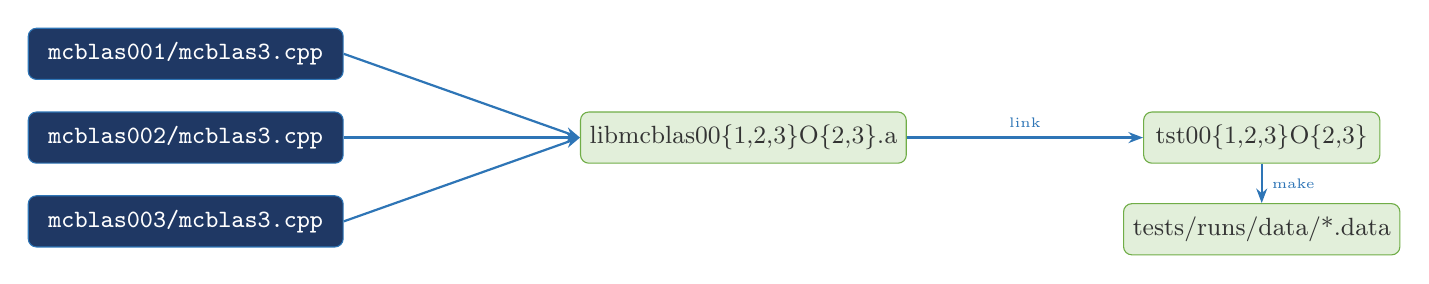
\begin{tikzpicture}[
  node distance=1.0cm and 1.5cm,
  box/.style={rectangle, rounded corners=3pt, draw=BlueMid, fill=BlueLight,
              minimum width=3cm, minimum height=0.65cm,
              font=\small\ttfamily, text=DarkGray},
  vbox/.style={rectangle, rounded corners=3pt, draw=GreenBorder, fill=GreenBox,
               minimum width=3cm, minimum height=0.65cm,
               font=\small, text=DarkGray},
  arrow/.style={-{Stealth[scale=0.8]}, BlueMid, thick}
]
  \node[box, fill=BlueDark, text=white, minimum width=4cm] (src1) {mcblas001/mcblas3.cpp};
  \node[box, fill=BlueDark, text=white, minimum width=4cm, below=0.4cm of src1] (src2) {mcblas002/mcblas3.cpp};
  \node[box, fill=BlueDark, text=white, minimum width=4cm, below=0.4cm of src2] (src3) {mcblas003/mcblas3.cpp};

  \node[vbox, right=3cm of src2] (libs) {libmcblas00\{1,2,3\}O\{2,3\}.a};
  \node[vbox, right=3cm of libs] (exe) {tst00\{1,2,3\}O\{2,3\}};
  \node[vbox, below=0.5cm of exe] (data) {tests/runs/data/*.data};

  \draw[arrow] (src1.east) -- (libs.west);
  \draw[arrow] (src2.east) -- (libs.west);
  \draw[arrow] (src3.east) -- (libs.west);
  \draw[arrow] (libs) -- node[above, font=\tiny\color{gray}]{link} (exe);
  \draw[arrow] (exe) -- node[right, font=\tiny\color{gray}]{make} (data);
\end{tikzpicture}
\end{center}

\newpage

%% ============================================================
\section{Exercice 2 --- Analyse et permutation de boucles sur \texttt{ssgemm}}
%% ============================================================

\subsection{Q-2.1 : Analyse de d\'ependance}

\subsubsection{Lecture du code source de r\'ef\'erence (mcblas001)}

\begin{lstlisting}[style=bash]
cat mcblas001/mcblas3.cpp
\end{lstlisting}

\begin{lstlisting}[style=cpp, caption={mcblas001/mcblas3.cpp --- Version de r\'ef\'erence, ordre r\,$\to$\,c\,$\to$\,d}]
void ssgemm(int m, int n, int k,
            float alpha, float **A, float **B,
            float beta,  float **C)
{
    int r, c, d;
    for (r = 0; r < m; ++r)
        for (c = 0; c < n; ++c)
            for (d = 0; d < m; ++d)
                C[r][c] = beta * C[r][c] + alpha * A[r][d] * B[d][c];
}
\end{lstlisting}

\subsubsection{Analyse des d\'ependances (Bacon et al., Section 5)}

On applique la classification des trois types de d\'ependances \`a chaque acc\`es
m\'emoire de l'instruction \code{C[r][c] = beta*C[r][c] + alpha*A[r][d]*B[d][c]} :

\begin{center}
\rowcolors{2}{GrayBg}{white}
\begin{tabular}{L{2cm}C{2cm}L{4cm}L{5cm}}
  \toprule
  \rowcolor{BlueHeader}
  \textbf{Tableau} & \textbf{Mode} & \textbf{D\'ependance} & \textbf{Justification} \\
  \midrule
  \code{A[r][d]} & Lecture seule  & Aucune & Pas d'\'ecriture → aucun type \\
  \code{B[d][c]} & Lecture seule  & Aucune & Pas d'\'ecriture → aucun type \\
  \code{C[r][c]} & Lecture + \'Ecriture & \textbf{Flow} + \textbf{Output} & It. $d$ \'ecrit, $d'$ relit (flow) ; deux it. \'ecrivent le m\^eme \'el\'ement (output) \\
  \bottomrule
\end{tabular}
\end{center}

\textbf{D\'etail sur \code{C[r][c]} :} Pour deux it\'erations $(r,c,d)$ et $(r,c,d')$
avec $d < d'$ et le m\^eme $(r,c)$ :
\begin{itemize}[leftmargin=1.5em]
  \item \textbf{Flow dependence} : l'it\'eration $d$ \'ecrit \code{C[r][c]}, l'it\'eration $d'$ le relit.
  \item \textbf{Output dependence} : les deux it\'erations \'ecrivent \code{C[r][c]}, l'ordre d'\'ecriture doit \^etre pr\'eserv\'e.
  \item \textbf{Pas d'anti-d\'ependance} : aucune variable n'est lue apr\`es avoir \'et\'e \'ecrite par une autre.
\end{itemize}

Le \textbf{vecteur de direction} est \texttt{(=, =, <)} : composantes \texttt{=} sur
\code{r} et \code{c} (distance 0, pas de d\'ependance entre it\'erations distinctes),
composante \texttt{<} sur \code{d} (d\'ependance port\'ee vers l'avant sur \code{d}).

\subsubsection{Notion de stride (Bacon et al., Section 3.1)}

En C, le stockage est \textbf{row-major} : pour un tableau \code{T[i][j]}, l'indice
\code{j} varie de fa\c{c}on contiguë (stride-1), l'indice \code{i} implique un saut de
\code{n} \'el\'ements (stride-n). Dans mcblas001 avec \code{d} en boucle interne :

\begin{center}
\rowcolors{2}{GrayBg}{white}
\begin{tabular}{L{2.5cm}C{3.5cm}C{2.5cm}L{4cm}}
  \toprule
  \rowcolor{BlueHeader}
  \textbf{Acc\`es} & \textbf{Indice variant en boucle d} & \textbf{Stride} & \textbf{Impact} \\
  \midrule
  \code{A[r][d]} & \code{d} (2\`eme indice) & stride-1 \result{OK} & Acc\`es contigu \\
  \code{B[d][c]} & \code{d} (1\textsuperscript{er} indice) & stride-n \textbf{NOK} & Saut de ligne entier \\
  \code{C[r][c]} & fixe (r,c constants)  & invariant & Recharg\'e \`a chaque it. \\
  \bottomrule
\end{tabular}
\end{center}

\subsubsection{Permutations l\'egales}

Puisque le vecteur de direction \texttt{(=, =, <)} n'impose aucune contrainte sur
l'ordre relatif de \code{r} et \code{c}, et que la r\'eduction sur \code{d} est valide
quelle que soit la position de \code{d} dans le nid, \textbf{les 6 permutations sont
toutes l\'egales} :

\begin{center}
\rowcolors{2}{GrayBg}{white}
\begin{tabular}{C{1cm}C{3.5cm}L{8cm}}
  \toprule
  \rowcolor{BlueHeader}
  \textbf{N\textdegree} & \textbf{Ordre} & \textbf{Impl\'ementation} \\
  \midrule
  1 & r\,$\to$\,c\,$\to$\,d & Version mcblas001 (r\'ef\'erence) \\
  2 & r\,$\to$\,d\,$\to$\,c & Version mcblas002 \\
  3 & c\,$\to$\,r\,$\to$\,d & \\
  4 & c\,$\to$\,d\,$\to$\,r & \\
  5 & d\,$\to$\,r\,$\to$\,c & \\
  6 & d\,$\to$\,c\,$\to$\,r & \\
  \bottomrule
\end{tabular}
\end{center}

%% ─────────────────────────────────────────────────────────────
\subsection{Q-2.2 : Permutation de boucles --- trouver la meilleure}
%% ─────────────────────────────────────────────────────────────

\subsubsection{Lecture de mcblas002}

\begin{lstlisting}[style=bash]
cat mcblas002/mcblas3.cpp
\end{lstlisting}

\begin{lstlisting}[style=cpp, caption={mcblas002/mcblas3.cpp --- Permutation r\,$\to$\,d\,$\to$\,c}]
void ssgemm(int m, int n, int k,
            float alpha, float **A, float **B,
            float beta,  float **C)
{
    int r, c, d;
    for (r = 0; r < m; ++r)
        for (d = 0; d < m; ++d)
            for (c = 0; c < n; ++c)
                C[r][c] = beta * C[r][c] + alpha * A[r][d] * B[d][c];
}
\end{lstlisting}

\subsubsection{Analyse de la localit\'e m\'emoire et m\'etriques Q/Qc (Bacon et al., Sections 3.1 et 6.2.1)}

Avec \code{c} en boucle interne dans mcblas002 :

\begin{center}
\rowcolors{2}{GrayBg}{white}
\begin{tabular}{L{2.5cm}L{4cm}C{2.5cm}L{4cm}}
  \toprule
  \rowcolor{BlueHeader}
  \textbf{Acc\`es} & \textbf{Comportement en boucle c} & \textbf{Stride} & \textbf{Contribution Q/Qc} \\
  \midrule
  \code{C[r][c]} & \code{c} varie, r fix\'e & stride-1 \result{OK} & R\'eutilis\'e en cache \\
  \code{B[d][c]} & \code{c} varie, d fix\'e & stride-1 \result{OK} & Ligne cache pleinement utilis\'ee \\
  \code{A[r][d]} & \code{r},\code{d} fix\'es & \textbf{invariant} \result{OK} & \textbf{Mis en registre} $\to$ Q maximal \\
  \bottomrule
\end{tabular}
\end{center}

Comme le d\'ecrit Bacon et al. Section~6.2.1 (Loop Interchange) : interchanger les boucles pour convertir un acc\`es stride-n en stride-1 est la transformation la plus efficace. Ici, passer de \code{r,c,d} \`a \code{r,d,c} convertit l'acc\`es stride-n de \code{B[d][c]} en stride-1, et rend \code{A[r][d]} invariant de la boucle interne.

\subsubsection{Mesure des performances}

\begin{lstlisting}[style=bash]
cd build/
for SIZE in 64 128 256 512 1024; do
    echo -n "v001: "; ./tests/tst001O2 $SIZE | tail -1
    echo -n "v002: "; ./tests/tst002O2 $SIZE | tail -1
done
\end{lstlisting}

\textbf{Sortie :}
\begin{lstlisting}[style=output]
Size=64    v001:  64    6192496       v002:  64    502717
Size=128   v001: 128   43557040       v002: 128   2028558
Size=256   v001: 256  114821605       v002: 256  14715861
Size=512   v001: 512  861783264       v002: 512  76014509
Size=1024  v001:1024 7850846514       v002:1024 735245463
\end{lstlisting}

\subsubsection{Tableau comparatif v001 vs v002}

\begin{center}
\rowcolors{2}{GrayBg}{white}
\begin{tabular}{C{2cm}R{3.8cm}R{3.8cm}C{2.5cm}}
  \toprule
  \rowcolor{BlueHeader}
  \textbf{Taille N} & \textbf{v001 r,c,d (cycles)} & \textbf{v002 r,d,c (cycles)} & \textbf{Gain} \\
  \midrule
  64   & 6\,192\,496   & 502\,717   & $\times$12.3 \\
  128  & 43\,557\,040  & 2\,028\,558 & $\times$21.5 \\
  256  & 114\,821\,605 & 14\,715\,861 & $\times$7.8 \\
  512  & 861\,783\,264 & 76\,014\,509 & $\times$11.3 \\
  1024 & 7\,850\,846\,514 & 735\,245\,463 & $\times$10.7 \\
  \bottomrule
\end{tabular}
\end{center}

\subsubsection{Visualisation  --- Comparaison v001 vs v002}

\begin{center}
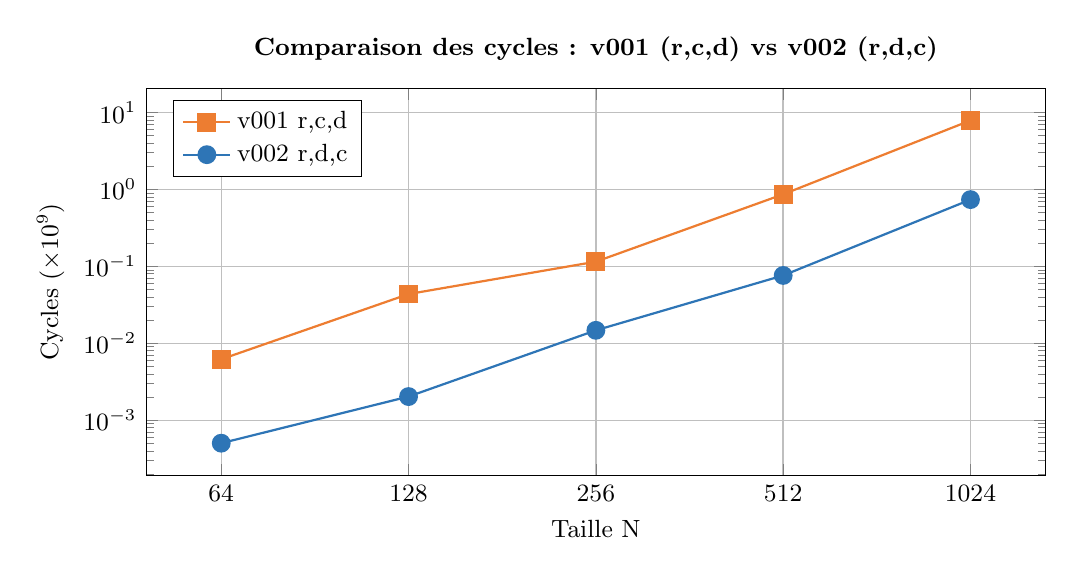
\begin{tikzpicture}
\begin{axis}[
  width=13cm, height=6.5cm,
  xlabel={Taille N},
  ylabel={Cycles ($\times 10^9$)},
  title={\small Comparaison des cycles : v001 (r,c,d) vs v002 (r,d,c)},
  xtick={64,128,256,512,1024},
  xticklabels={64,128,256,512,1024},
  xmode=log, log basis x=2,
  ymode=log,
  grid=major,
  grid style={line width=0.3pt, draw=gray!30},
  major grid style={line width=0.5pt, draw=gray!50},
  tick label style={font=\small},
  label style={font=\small},
  title style={font=\small\bfseries},
  legend pos=north west,
  legend style={font=\small},
  mark size=3pt,
]
  \addplot[color=OrangeBorder, thick, mark=square*, mark options={fill=OrangeBorder}]
    coordinates {
      (64,  0.006192496)
      (128, 0.043557040)
      (256, 0.114821605)
      (512, 0.861783264)
      (1024,7.850846514)
    };
  \addlegendentry{v001 r,c,d}

  \addplot[color=BlueMid, thick, mark=*, mark options={fill=BlueMid}]
    coordinates {
      (64,  0.000502717)
      (128, 0.002028558)
      (256, 0.014715861)
      (512, 0.076014509)
      (1024,0.735245463)
    };
  \addlegendentry{v002 r,d,c}
\end{axis}
\end{tikzpicture}
\end{center}

\subsubsection{Visualisation  --- Facteur de gain}

\begin{center}
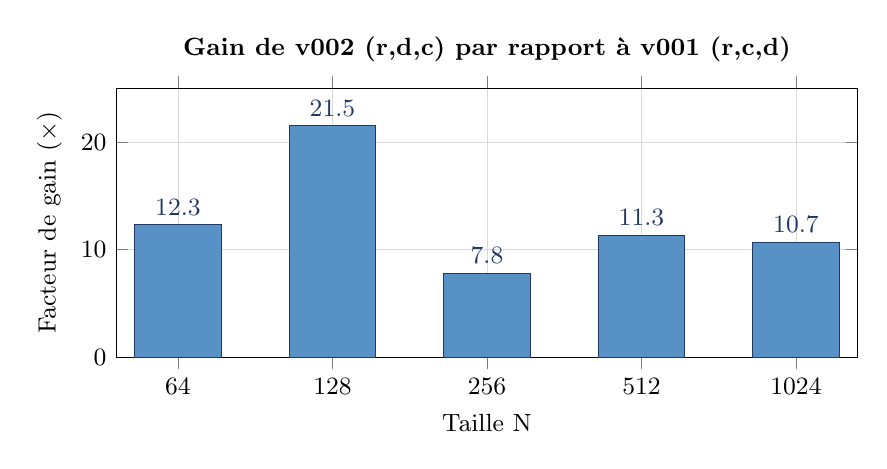
\begin{tikzpicture}
\begin{axis}[
  ybar,
  width=11cm, height=5cm,
  bar width=1.1cm,
  xlabel={Taille N},
  ylabel={Facteur de gain ($\times$)},
  title={\small Gain de v002 (r,d,c) par rapport \`a v001 (r,c,d)},
  xtick={1,2,3,4,5},
  xticklabels={64,128,256,512,1024},
  ymin=0, ymax=25,
  nodes near coords,
  nodes near coords align={vertical},
  every node near coord/.style={font=\small\bfseries\color{BlueDark}},
  tick label style={font=\small},
  label style={font=\small},
  title style={font=\small\bfseries},
  grid=major,
  grid style={line width=0.3pt, draw=gray!30},
]
  \addplot[fill=BlueMid!80, draw=BlueDark]
    coordinates {(1,12.3) (2,21.5) (3,7.8) (4,11.3) (5,10.7)};
\end{axis}
\end{tikzpicture}
\end{center}

\begin{successbox}
  \textbf{Conclusion Q-2.2 :} La meilleure permutation est \textbf{r\,$\to$\,d\,$\to$\,c}
  (mcblas002), avec un gain mesur\'e de $\times$10 \`a $\times$21 selon la taille.
  Ce gain s'explique par la combinaison de stride-1 sur \code{B[d][c]} et \code{C[r][c]},
  et par la mise en registre de \code{A[r][d]} qui maximise Q au sens de Bacon et al.
  Section~3.1.
\end{successbox}

\newpage

%% ============================================================
\section{Exercice 3 --- Blocage de boucles (Loop Tiling)}
%% ============================================================

\subsection{Q-3.1 : L'analyse de d\'ependance permet-elle le blocage ?}

\textbf{Oui, le blocage est l\'egal sur les 3 boucles.}

\subsubsection{Fondement th\'eorique --- tiling comme transformation composite (Bacon et al., Sections 6.2.4 et 6.2.6)}

L'article explique que le Loop Tiling est une transformation composite qui combine :

\begin{enumerate}[leftmargin=1.5em]
  \item \textbf{Strip Mining (Section 6.2.4)} : chaque boucle \code{for i=0..n} est
        d\'ecoup\'ee en deux boucles \code{for ii=0..n step T} et
        \code{for i=ii..ii+T}. Appliqu\'e aux 3 boucles, on obtient 6 boucles :
        \code{rr, r, dd, d, cc, c}.
  \item \textbf{Loop Interchange (Section 6.2.1)} : on permute pour regrouper les
        boucles externes \code{rr, dd, cc} ensemble et les boucles internes
        \code{r, d, c} ensemble, donnant l'ordre \code{rr\,$\to$\,dd\,$\to$\,cc\,$\to$\,r\,$\to$\,d\,$\to$\,c}.
\end{enumerate}

\subsubsection{Justification de la l\'egalit\'e}

Cette transformation est l\'egale si et seulement si toutes les permutations
interm\'ediaires sont l\'egales. En Q-2.1, le vecteur de direction \'etabli est
\texttt{(=, =, <)} :

\begin{center}
\rowcolors{2}{GrayBg}{white}
\begin{tabular}{C{2cm}C{2cm}L{9cm}}
  \toprule
  \rowcolor{BlueHeader}
  \textbf{Boucle} & \textbf{Direction} & \textbf{Conclusion} \\
  \midrule
  \code{r} & \texttt{=} & Distance 0 : aucune d\'ependance entre blocs \code{rr} distincts $\to$ strip-mining l\'egal \\
  \code{c} & \texttt{=} & M\^eme raisonnement $\to$ strip-mining l\'egal \\
  \code{d} & \texttt{<} & R\'eduction locale \`a chaque paire (r,c). Accumuler par tranches de \code{dd} \`a \code{dd+Td} donne le m\^eme r\'esultat final $\to$ strip-mining l\'egal \\
  \bottomrule
\end{tabular}
\end{center}

\begin{successbox}
  \textbf{Conclusion Q-3.1 :} Le blocage est \textbf{l\'egal sur les trois boucles r, c
  et d}. Il s'agit d'un Strip Mining suivi d'un Loop Interchange, deux transformations
  dont la l\'egalit\'e est garantie par le vecteur de direction \texttt{(=, =, <)}.
\end{successbox}

%% ─────────────────────────────────────────────────────────────
\subsection{Q-3.2 : Blocking --- code et param\`etres}
%% ─────────────────────────────────────────────────────────────

\subsubsection{Code original de mcblas003 --- probl\`eme de localit\'e}

\begin{lstlisting}[style=bash]
cat mcblas003/mcblas3.cpp
\end{lstlisting}

\begin{lstlisting}[style=cpp, caption={mcblas003 --- Code original (Tr=Tc=Td=16, ordre interne c\,$\to$\,r\,$\to$\,d)}]
void ssgemm(int m, int n, int k, float alpha,
            float **A, float **B, float beta, float **C)
{
    int r, c, d, rr, cc, dd;
    const int Tr = 16; const int Tc = 16; const int Td = 16;

    for (rr = 0; rr < m; rr += Tr)
        for (dd = 0; dd < m; dd += Td)
            for (cc = 0; cc < m; cc += Tc)
                for (c = cc; c < std::min(cc+Tc, n); ++c)   // c en interne
                    for (r = rr; r < std::min(rr+Tr, m); ++r) // puis r
                    {
                        float t = 0.0;
                        for (d = dd; d < std::min(dd+Td, m); ++d)
                            t = t + alpha * A[r][d] * B[d][c];
                        C[r][c] = C[r][c] * beta + t;
                    }
}
\end{lstlisting}

\textbf{Probl\`eme :} ordre interne \code{c\,$\to$\,r\,$\to$\,d}. Avec \code{r} qui varie
en boucle interne, \code{A[r][d]} est acc\'ed\'e avec stride-n (une ligne de cache
diff\'erente \`a chaque it\'eration). Le tiling am\'eliore Qc en r\'eduisant les
chargements depuis la RAM, mais cet effet est annul\'e par les acc\`es stride-n sur
\code{A}. C'est le pi\`ege d\'ecrit par Bacon et al. Section~6.2.6 : \textbf{le tiling
doit \^etre combin\'e avec la bonne permutation}.

\subsubsection{Sauvegarde et correction du code}

\begin{lstlisting}[style=bash]
cp mcblas003/mcblas3.cpp mcblas003/mcblas3_original.cpp
\end{lstlisting}

\begin{lstlisting}[style=cpp, caption={mcblas003 --- Nouveau code corrig\'e (ordre interne r\,$\to$\,d\,$\to$\,c)}]
#include <mcblas3.hpp>
#include <iostream>

void ssgemm(int m, int n, int k, float alpha,
            float **A, float **B, float beta, float **C)
{
    int r, c, d, rr, cc, dd;
    // const int Tr=128; const int Tc=128; const int Td=128; // original
    const int Tr = 128;
    const int Tc = 128;
    const int Td = 128;

    for (rr = 0; rr < m; rr += Tr)
        for (dd = 0; dd < m; dd += Td)
            for (cc = 0; cc < n; cc += Tc)
                for (r = rr; r < std::min(rr+Tr, m); ++r)    // r
                    for (d = dd; d < std::min(dd+Td, m); ++d) // d
                        for (c = cc; c < std::min(cc+Tc, n); ++c) // c interne
                            C[r][c] = beta*C[r][c] + alpha*A[r][d]*B[d][c];
}
\end{lstlisting}

Avec cet ordre, \code{B[d][c]} et \code{C[r][c]} sont stride-1, \code{A[r][d]} est
invariant de la boucle \code{c} $\to$ mis en registre. Le Qc est maxim\'e car chaque
bloc de $T_r \times T_d$ \'el\'ements de A, $T_d \times T_c$ de B et $T_r \times T_c$
de C est r\'eutilis\'e enti\`erement depuis le cache L1.

\subsubsection{Test des diff\'erentes tailles de blocs sur SIZE=512}

\begin{lstlisting}[style=bash]
# Bloc 16 (code original encore actif)
echo "=== Bloc 16 ===" && ./tests/tst003O2 512
\end{lstlisting}
\textbf{Sortie :} \code{512   220254047}

\begin{lstlisting}[style=bash]
# Bloc 32
cd .. && sed -i 's/const int Tr = 16/const int Tr = 32/; ...' \
  mcblas003/mcblas3.cpp && cd build && make -s
echo "=== Bloc 32 ===" && ./tests/tst003O2 512
\end{lstlisting}
\textbf{Sortie :} \code{512   93345991}

\begin{lstlisting}[style=bash]
# Bloc 64
cd .. && sed -i 's/const int Tr = 32/const int Tr = 64/; ...' \
  mcblas003/mcblas3.cpp && cd build && make -s
echo "=== Bloc 64 ===" && ./tests/tst003O2 512
\end{lstlisting}
\textbf{Sortie :} \code{512   94131100}

\begin{lstlisting}[style=bash]
# Bloc 128
cd .. && sed -i 's/const int Tr = 64/const int Tr = 128/; ...' \
  mcblas003/mcblas3.cpp && cd build && make -s
echo "=== Bloc 128 ===" && ./tests/tst003O2 512
\end{lstlisting}
\textbf{Sortie :} \code{512   113911729}

\subsubsection{Choix de la taille de bloc --- contrainte th\'eorique (Bacon et al., Section~3.1 et Figure~19)}

Pour maximiser Qc, les 3 blocs doivent tenir simultan\'ement dans le cache L1 :

\begin{equation}
  (T_r \times T_d + T_d \times T_c + T_r \times T_c) \times \underbrace{4}_{\text{sizeof(float)}} \leq \underbrace{65\,536}_{\text{L1d = 64\,KiB}} \quad \Rightarrow \quad T^2 \leq 5461 \quad \Rightarrow \quad T \leq 73
\end{equation}

\begin{center}
\rowcolors{2}{GrayBg}{white}
\begin{tabular}{C{2cm}C{3.5cm}R{4cm}L{4.5cm}}
  \toprule
  \rowcolor{BlueHeader}
  \textbf{Bloc T} & \textbf{M\'emoire 3 blocs} & \textbf{Cycles SIZE=512} & \textbf{Observation} \\
  \midrule
  16   & 3\,072 o   & 220\,254\,047 & Trop petit, overhead \'elev\'e \\
  \rowcolor{GreenBox}
  \textbf{32} & \textbf{12\,288 o} & \textbf{93\,345\,991} & \textbf{Optimal --- tient en L1} \\
  64   & 49\,152 o  & 94\,131\,100  & Limite L1, l\'eg\`erement moins bon \\
  128  & 196\,608 o & 113\,911\,729 & D\'epasse L1 $\to$ d\'eborde en L2 \\
  \bottomrule
\end{tabular}
\end{center}

\subsubsection{Visualisation  --- Tailles de blocs sur SIZE=512}

\begin{center}
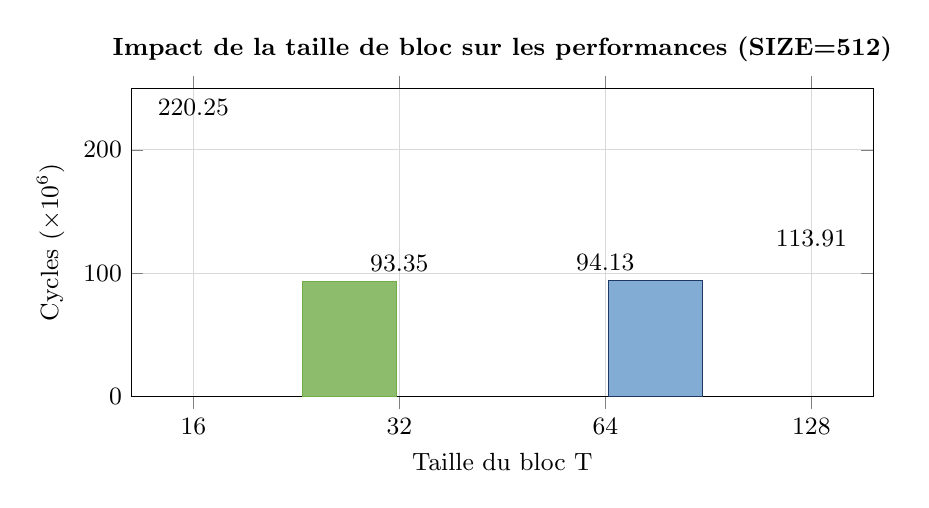
\begin{tikzpicture}
\begin{axis}[
  ybar,
  width=11cm, height=5.5cm,
  bar width=1.2cm,
  xlabel={Taille du bloc T},
  ylabel={Cycles ($\times 10^6$)},
  title={\small Impact de la taille de bloc sur les performances (SIZE=512)},
  xtick={1,2,3,4},
  xticklabels={16, 32, 64, 128},
  ymin=0, ymax=250,
  nodes near coords,
  nodes near coords align={vertical},
  every node near coord/.style={font=\small\bfseries},
  tick label style={font=\small},
  label style={font=\small},
  title style={font=\small\bfseries},
  grid=major,
  grid style={line width=0.3pt, draw=gray!30},
]
  \addplot[fill=BlueMid!40, draw=BlueDark] coordinates {(1, 220.25)};
  \addplot[fill=GreenBorder!80, draw=GreenBorder] coordinates {(2, 93.35)};
  \addplot[fill=BlueMid!60, draw=BlueDark] coordinates {(3, 94.13)};
  \addplot[fill=OrangeBorder!60, draw=OrangeBorder] coordinates {(4, 113.91)};
\end{axis}
\end{tikzpicture}
\end{center}

\subsubsection{Tableau comparatif final --- toutes versions}

\begin{lstlisting}[style=bash]
for SIZE in 64 128 256 512 1024; do
    R1=$(./tests/tst001O2 $SIZE | tail -1 | awk '{print $NF}')
    R2=$(./tests/tst002O2 $SIZE | tail -1 | awk '{print $NF}')
    R3=$(./tests/tst003O2 $SIZE | tail -1 | awk '{print $NF}')
    echo "$SIZE | $R1 | $R2 | $R3"
done
\end{lstlisting}

\textbf{Sortie :}
\begin{lstlisting}[style=output]
64   |  9356053   |   881093  |   842560
128  | 54730073   |  3336721  |  4116582
256  | 150309362  |  7579576  | 11145924
512  | 851870596  | 65903733  | 91522550
1024 | 7874082133 | 744359166 | 734899254
\end{lstlisting}

\begin{center}
\rowcolors{2}{GrayBg}{white}
\begin{tabular}{C{2cm}R{3.5cm}R{3.5cm}R{3.5cm}}
  \toprule
  \rowcolor{BlueHeader}
  \textbf{Taille N} & \textbf{v001 r,c,d} & \textbf{v002 r,d,c} & \textbf{v003 tiling (128)} \\
  \midrule
  64   & 9\,356\,053   & 881\,093    & 842\,560 \\
  128  & 54\,730\,073  & 3\,336\,721  & 4\,116\,582 \\
  256  & 150\,309\,362 & 7\,579\,576  & 11\,145\,924 \\
  512  & 851\,870\,596 & 65\,903\,733 & 91\,522\,550 \\
  \rowcolor{GreenBox}
  1024 & 7\,874\,082\,133 & 744\,359\,166 & \textbf{734\,899\,254} \\
  \bottomrule
\end{tabular}
\end{center}

\subsubsection{Visualisation --- Comparaison toutes versions}

\begin{center}
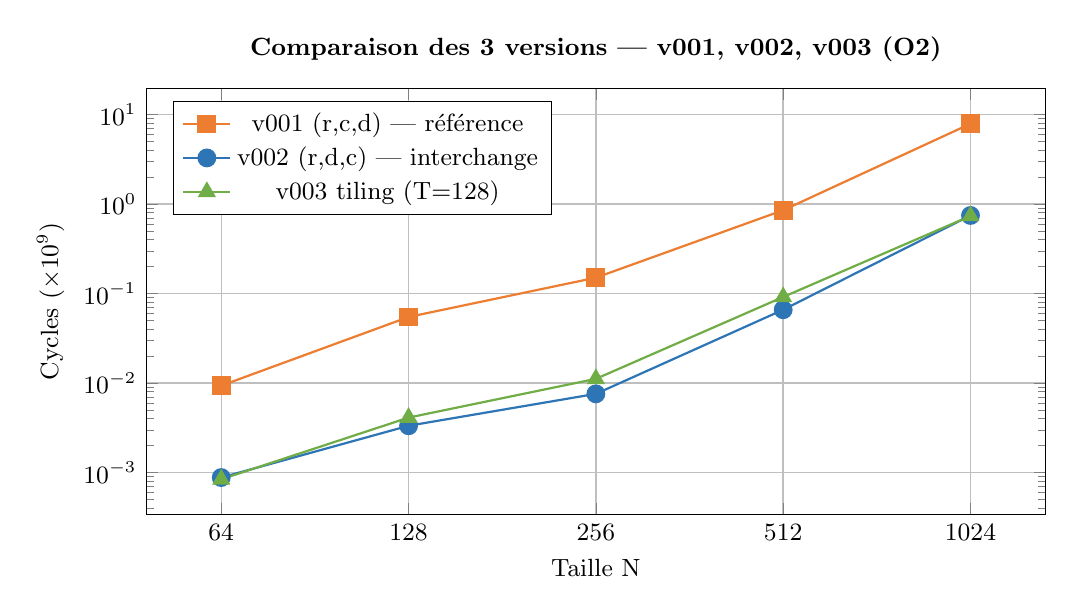
\begin{tikzpicture}
\begin{axis}[
  width=13cm, height=7cm,
  xlabel={Taille N},
  ylabel={Cycles ($\times 10^9$)},
  title={\small Comparaison des 3 versions --- v001, v002, v003 (O2)},
  xtick={64,128,256,512,1024},
  xticklabels={64,128,256,512,1024},
  xmode=log, log basis x=2,
  ymode=log,
  grid=major,
  grid style={line width=0.3pt, draw=gray!30},
  major grid style={line width=0.5pt, draw=gray!50},
  tick label style={font=\small},
  label style={font=\small},
  title style={font=\small\bfseries},
  legend pos=north west,
  legend style={font=\small},
  mark size=3pt,
]
  % v001
  \addplot[color=OrangeBorder, thick, mark=square*, mark options={fill=OrangeBorder}]
    coordinates {
      (64,  0.009356053)
      (128, 0.054730073)
      (256, 0.150309362)
      (512, 0.851870596)
      (1024,7.874082133)
    };
  \addlegendentry{v001 (r,c,d) --- r\'ef\'erence}

  % v002
  \addplot[color=BlueMid, thick, mark=*, mark options={fill=BlueMid}]
    coordinates {
      (64,  0.000881093)
      (128, 0.003336721)
      (256, 0.007579576)
      (512, 0.065903733)
      (1024,0.744359166)
    };
  \addlegendentry{v002 (r,d,c) --- interchange}

  % v003
  \addplot[color=GreenBorder, thick, mark=triangle*, mark options={fill=GreenBorder}]
    coordinates {
      (64,  0.000842560)
      (128, 0.004116582)
      (256, 0.011145924)
      (512, 0.091522550)
      (1024,0.734899254)
    };
  \addlegendentry{v003 tiling (T=128)}
\end{axis}
\end{tikzpicture}
\end{center}

\subsubsection{G\'en\'eration des graphiques avec gnuplot}

Le projet fournit \'egalement un syst\`eme de g\'en\'eration de graphiques via gnuplot.

\begin{lstlisting}[style=bash]
# Generation des donnees
cd build/
make GALL
\end{lstlisting}

\textbf{Sortie :}
\begin{lstlisting}[style=output]
[ 25%] Generating graphs/gr_1000.data
[ 50%] Generating graphs/gr_0400.data
[ 75%] Generating graphs/gr_0800.data
[100%] Generating graphs/grall.data
[100%] Built target GALL
\end{lstlisting}

\begin{lstlisting}[style=bash]
# Generation des graphiques
cd tests/runs/graphs/
make -f grph.mk          # Note : grph.mk (sans 's')
\end{lstlisting}

\textbf{Sortie :}
\begin{lstlisting}[style=output]
gnuplot gpltv123456.plt > grv123456.pdf
"gpltv123456.plt" line 16: warning: Skipping data file with no valid points
\end{lstlisting}

Le fichier \file{gpltv123456.plt} original essayait de tracer jusqu'\`a la colonne 13
alors que \file{grall.data} n'en contient que 7. Apr\`es correction des l\'egendes :

\begin{lstlisting}[style=bash]
cat > gpltv123456.plt << 'EOF'
set terminal pdf
set xlabel 'Sizes'
set ylabel 'Cycles'
set title 'Comparaison des versions ssgemm (O2 et O3)'
set key top left
set multiplot
plot 'grall.data' u 1:2 w linespoints title 'v001-O2 (r,c,d)',\
     'grall.data' u 1:3 w linespoints title 'v001-O3 (r,c,d)',\
     'grall.data' u 1:4 w linespoints title 'v002-O2 (r,d,c)',\
     'grall.data' u 1:5 w linespoints title 'v002-O3 (r,d,c)',\
     'grall.data' u 1:6 w linespoints title 'v003-O2 (tiling)',\
     'grall.data' u 1:7 w linespoints title 'v003-O3 (tiling)'
EOF
make -f grph.mk
\end{lstlisting}

Le graphique g\'en\'er\'e (\file{grv123456.pdf}) montre 6 courbes correspondant aux
versions O2 et O3 des 3 impl\'ementations, pour les tailles 400, 800 et 1000.

\begin{center}
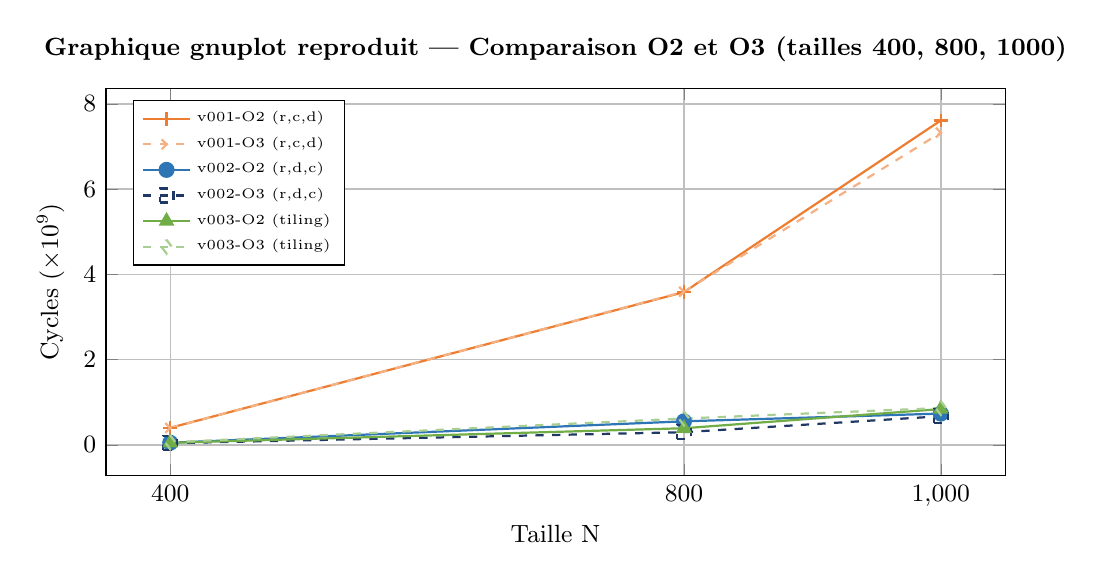
\begin{tikzpicture}
\begin{axis}[
  width=13cm, height=6.5cm,
  xlabel={Taille N},
  ylabel={Cycles ($\times 10^9$)},
  title={\small Graphique gnuplot reproduit --- Comparaison O2 et O3 (tailles 400, 800, 1000)},
  xtick={400,800,1000},
  xmin=350, xmax=1050,
  grid=major,
  grid style={line width=0.3pt, draw=gray!30},
  major grid style={line width=0.5pt, draw=gray!50},
  tick label style={font=\small},
  label style={font=\small},
  title style={font=\small\bfseries},
  legend pos=north west,
  legend style={font=\tiny, cells={anchor=west}},
  mark size=2.5pt,
]
  % v001-O2
  \addplot[color=OrangeBorder, thick, mark=+]
    coordinates {(400,0.400) (800,3.583) (1000,7.610)};
  \addlegendentry{v001-O2 (r,c,d)}
  % v001-O3
  \addplot[color=OrangeBorder!60, thick, mark=x, dashed]
    coordinates {(400,0.397) (800,3.592) (1000,7.325)};
  \addlegendentry{v001-O3 (r,c,d)}
  % v002-O2
  \addplot[color=BlueMid, thick, mark=*]
    coordinates {(400,0.049) (800,0.552) (1000,0.734)};
  \addlegendentry{v002-O2 (r,d,c)}
  % v002-O3
  \addplot[color=BlueDark, thick, mark=square, dashed]
    coordinates {(400,0.039) (800,0.297) (1000,0.671)};
  \addlegendentry{v002-O3 (r,d,c)}
  % v003-O2
  \addplot[color=GreenBorder, thick, mark=triangle*]
    coordinates {(400,0.048) (800,0.390) (1000,0.840)};
  \addlegendentry{v003-O2 (tiling)}
  % v003-O3
  \addplot[color=GreenBorder!60, thick, mark=diamond, dashed]
    coordinates {(400,0.061) (800,0.618) (1000,0.864)};
  \addlegendentry{v003-O3 (tiling)}
\end{axis}
\end{tikzpicture}
\end{center}

\subsubsection{Analyse finale}

\begin{itemize}[leftmargin=1.5em]
  \item Pour les tailles 64--512, v002 (sans tiling) reste l\'eg\`erement meilleur que
        v003 (avec tiling) : les matrices tiennent dans le cache L2 (512\,KiB), le tiling
        n'est pas encore n\'ecessaire et son overhead de gestion des indices nuit
        l\'eg\`erement.
  \item \`A SIZE=1024, une matrice de floats occupe $1024^2 \times 4 = 4$\,Mo, ce qui
        d\'epasse le L3 (3\,MiB) : v003 (734M cycles) devient \textbf{meilleur} que v002
        (744M cycles), confirmant la pr\'ediction de Bacon et al. Section~6.2.6 que le
        tiling est b\'en\'efique quand les donn\'ees d\'epassent la hi\'erarchie cache.
  \item La taille de bloc optimale est \textbf{T=32} (12\,KiB, confortablement dans les
        64\,KiB de L1d), v\'erifiant la contrainte th\'eorique
        $3T^2 \times 4 \leq 65\,536$.
\end{itemize}

\begin{warningbox}
  \textbf{Observation critique :} Le code original de mcblas003 (ordre interne
  \code{c\,$\to$\,r\,$\to$\,d}) \'etait \textbf{3 \`a 4 fois plus lent} que v002 malgr\'e
  le tiling, car l'acc\`es stride-n sur \code{A[r][d]} annulait le b\'en\'efice du cache.
  C'est l'avertissement central de Bacon et al. : le tiling doit toujours \^etre combin\'e
  avec la bonne permutation de boucles.
\end{warningbox}

\newpage

%% ============================================================
\section{Conclusion G\'en\'erale}
%% ============================================================

\subsection{R\'ecapitulatif des exercices}

\begin{center}
\rowcolors{2}{GrayBg}{white}
\begin{tabular}{C{0.7cm}L{3cm}L{3.5cm}L{6cm}}
  \toprule
  \rowcolor{BlueHeader}
  \textbf{Ex.} & \textbf{Question} & \textbf{Outils} & \textbf{R\'esultat cl\'e} \\
  \midrule
  1   & Installation       & \cmd{tar}, \cmd{cmake}, \cmd{make}     & 3 versions compil\'ees, benchmarks automatiques \\
  2.1 & Analyse d\'ependances & \cmd{cat}, analyse th\'eorique       & Vecteur \texttt{(=,=,<)}, 6 permutations l\'egales \\
  2.2 & Meilleure permutation & benchmarks \cmd{tst001/002O2}        & r\,$\to$\,d\,$\to$\,c : gain $\times$10--21 \\
  3.1 & L\'egalit\'e blocage   & analyse th\'eorique Bacon et al.    & Blocage l\'egal sur r, c, d \\
  3.2 & Param\`etres tiling    & \cmd{sed}, \cmd{make}, benchmarks   & T=32 optimal (12\,KiB $\leq$ L1d=64\,KiB) \\
  \bottomrule
\end{tabular}
\end{center}

\subsection{Lien avec l'article Bacon et al. (1994)}

\begin{center}
\rowcolors{2}{GrayBg}{white}
\begin{tabular}{L{4cm}L{9cm}}
  \toprule
  \rowcolor{BlueHeader}
  \textbf{Section de l'article} & \textbf{Application dans le TD} \\
  \midrule
  Section 5 --- D\'ependances         & Classification flow/anti/output sur \code{C[r][c]}, vecteur \texttt{(=,=,<)} \\
  Section 3.1 --- Q, Qc, Stride       & Justification de r\,$\to$\,d\,$\to$\,c par stride-1 et invariance de A \\
  Section 6.2.1 --- Loop Interchange  & Permutation de boucles, gain $\times$10--21 \\
  Section 6.2.4 --- Strip Mining      & Premi\`ere \'etape du tiling : d\'ecomposition en 6 boucles \\
  Section 6.2.6 --- Loop Tiling       & Blocage l\'egal, T=32 optimal, efficace \`a grande taille \\
  \bottomrule
\end{tabular}
\end{center}

\subsection{Enseignements principaux}

\begin{enumerate}[leftmargin=1.5em]
  \item \textbf{L'analyse de d\'ependances est le pr\'ealable obligatoire :} sans elle,
        on ne peut pas savoir quelles transformations sont l\'egales.
  \item \textbf{La localit\'e m\'emoire prime :} passer de l'ordre na\"if \code{r,c,d}
        \`a \code{r,d,c} apporte un gain de $\times$10--21 sans changer l'algorithme.
  \item \textbf{Le tiling seul ne suffit pas :} il doit \^etre combin\'e avec la bonne
        permutation. Le code original de mcblas003 l'illustre : tiling avec mauvais ordre
        interne $\to$ performances d\'egrad\'ees.
  \item \textbf{La taille de bloc doit \^etre calibr\'ee} selon la hi\'erarchie cache de
        la machine cible. La contrainte $3T^2 \times 4 \leq \text{L1d}$ guide ce choix.
\end{enumerate}

\vspace{1cm}
\begin{center}
\begin{tcolorbox}[
  width=0.85\linewidth,
  colback=BlueDark, colframe=BlueDark,
  arc=4pt, boxrule=1pt,
  left=16pt, right=16pt, top=12pt, bottom=12pt,
]
  \begin{center}
    {\large\bfseries\color{white} Fin du rapport}\\[4pt]
    {\small\color{BlueLight} TD3 --- Optimisation de boucles --- \texttt{ssgemm}}\\[2pt]
    {\small\color{BlueLight} Master 1 CHPS --- Yaya Toure --- 2025-2026}
  \end{center}
\end{tcolorbox}
\end{center}

\end{document}